\subsection{Obtained spectra}
% \begin{figure}[htbp]
  \centering
  \includegraphics[width=8cm]{../pic/Dron/All_CS_woK0.eps}
  \caption{
    The obtained cross sections are plotted simultaneously in this figure.
    The $d(K^-, n)"\pi^-\Sigma^+$, $d(K^-, n)"\pi^+\Sigma^-"$, and $d(K^-, p)"\pi^- \Sigma^0"$ plot as red, blue, and orange, lines respectively.
    The green virtical line indicates the $\bar{K}N$ threshold.
  }
  \label{fig:all_CS}
\end{figure}

\begin{figure}[htbp]
  \centering
  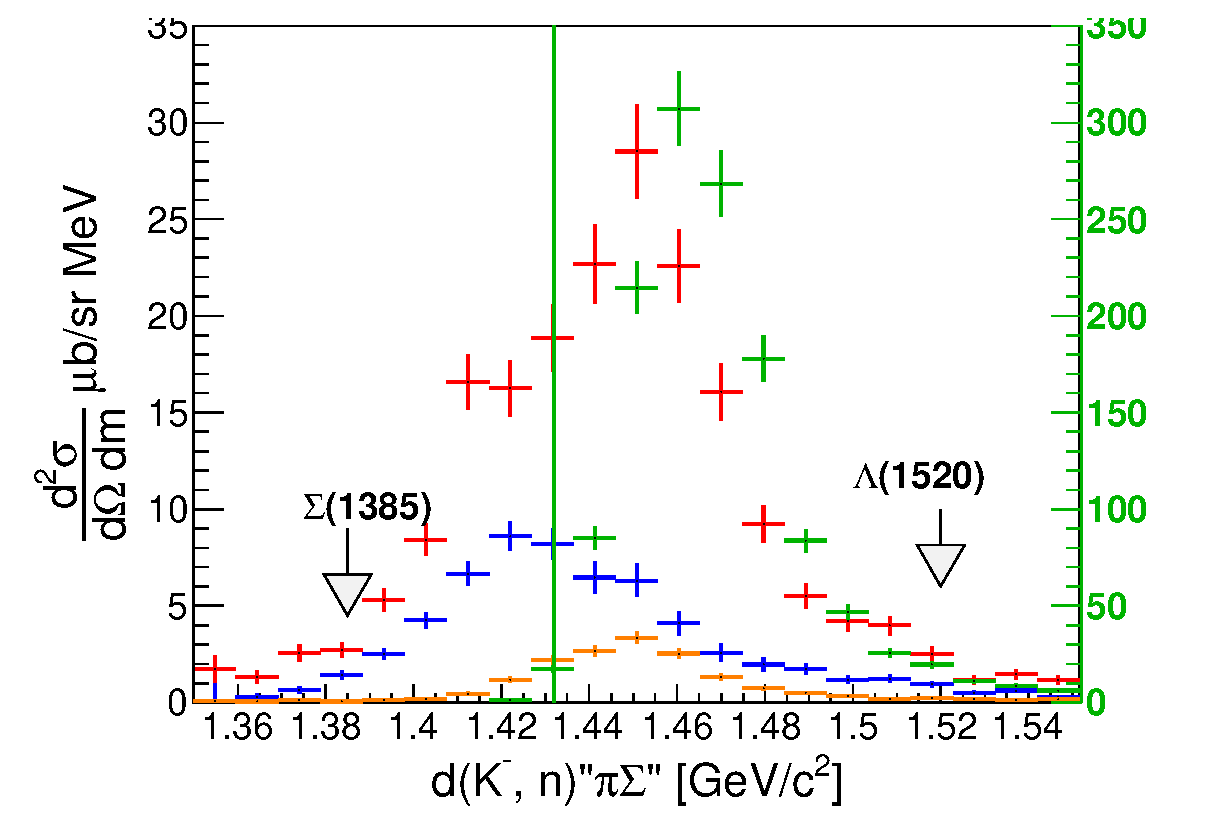
\includegraphics[width=8cm]{../pic/Dron/All_CS.eps}
  \caption{
    The obtained cross sections are plotted simultaneously in this figure.
    The $d(K^-, n)"\pi^-\Sigma^+$, $d(K^-, n)"\pi^+\Sigma^-"$, $d(K^-, n)"n K^0"$, and $d(K^-, p)"\pi^- \Sigma^0"$ plot as red, blue, green, and orange, lines respectively.
    The $d(K^-, n)"n K^0"$ is scaled to 1/10.
    The green virtical line indicates the $\bar{K}N$ threshold.
  }
  \label{fig:all_CS}
\end{figure}


In this subsection we discuss the physical meaning of the obtained spectra, for which we simultaneously plot the obtained spectra in Figure.\ref{fig:all_CS}.
In this figure, $d(K^-, n)"n K^0"$ is scaled to 1/10 for comparison with 1-step quasi-elastic scattering.

The $d(K^-,n)"nK^0"$ spectra do not contain information below the $\bar{K}N$ threshold but are suitable for studying the $d(K^-, n)$ reaction.
This spectrum is similar to the bump structure of the so-called quasi-elastic scattering.
This spectrum contains about 12\% of the 2-step reaction described in the previous section.
Since the missing mass of $d(K^-,n)$ is determined by the $K^- N \rightarrow \bar{K}N$ scattering of the first reaction, this spectrum has almost the same shape as quasi-elastic scattering.
The strength of the 2-step at the quasi-elastic scattering bump is $35 mb/\Omega \cdot \mbox{MeV}$, which is consistent with $d(K^-, N)"\pi \Sigma"$ in order.

Next,
we discuss the $d(K^-, N)\pi \Sigma$ including the scattering amplitude below the $\bar{K}N$ threshold.
There is an $I=1$ p-wave state, $\Sigma(1385)$, and an $I=0$ d-wave state, $\Lambda(1520)$, near the $\bar{K}N$ threshold.
However, the pure $I=1$ $d(K^-, p)"\pi^-\Sigma^0"$ spectrum has no structure around the region of $\Sigma(1385)$,
and the $d(K^-, n)"\pi^{\mp} \Sigma^{\pm}"$ spectrum contributed from $I=0$ and $I=1$ has no structure around $\Sigma(1385)$ and $\Lambda(1520)$.
This means that in the $d(K^-, N)"\pi \Sigma"$ reaction, the $P$-wave, $D$-wave, and higher-order waves are suppressed and the $S$-wave is dominant.

The $d(K^-, p)\pi^- \Sigma^0$ spectrum resembles the bump structure of quasi-elastic scattering.
In other words, the spectrum strongly reflects the first $K^-N \rightarrow \bar{K}N$ scattering
because there is no pole near the $\bar{K}N$ threshold and there is no significant change in the amplitude of the second $\bar{K}N\rightarrow \pi\Sigma$ scattering at $I=1$.

On the other hand, an excess strength below the $\bar{K}N$ threxshold is observed in the $d(K-, n)"\pi^{\mp} \Sigma^{\pm}"$ spectrum,
which is considered to be a contribution from the $I=0$ amplitude of second $\bar{K}N\rightarrow \pi \Sigma$ scattering.
The $I=0$ and $I=1$ interference terms at the second $\bar{K}N \rightarrow \pi \Sigma$ scattering amplitude appears as the difference between the $\pi-\Sigma^+$ and $\pi^+ \Sigma^-$ spectra.
This difference is observed in the obtained $d(K^-, n)"\pi^{\mp} \Sigma^{\pm}"$ spectrum, whose behavior changes dramatically above and below the $\bar{K}N$ threshold.
The scattering amplitude changes dramatically at the poles. 
This effect is emphized by the scattering particle mass threshold.
Thus, the observed interference term suggests that the pole exists just below the $\bar{K}N$ threshold.
